\documentclass{article}

\usepackage[T1]{fontenc}

\usepackage[affil-it]{authblk}

\usepackage[USenglish,american]{babel}
\usepackage[pdftex]{graphicx}
\usepackage{epstopdf}

\usepackage{cite}

\usepackage{amsfonts,amsmath,amsthm,amssymb}

\usepackage{tikz,pgf}
\usetikzlibrary{fit}

\usepackage{csvsimple}

%\pagestyle{empty}
\setlength{\parindent}{0mm}
\usepackage[letterpaper, margin=1in]{geometry}
%\usepackage{showframe}

\usepackage{multicol}
\usepackage{enumerate}

\usepackage{verbatim}
\usepackage{listings}

\usepackage{color}

%%
%% Julia definition (c) 2014 Jubobs
%%
\lstdefinelanguage{Julia}%
  {morekeywords={abstract,break,case,catch,const,continue,do,else,elseif,%
      end,export,false,for,function,immutable,import,importall,if,in,%
      macro,module,otherwise,quote,return,switch,true,try,type,typealias,%
      using,while},%
   sensitive=true,%
   alsoother={$},%
   morecomment=[l]\#,%
   morecomment=[n]{\#=}{=\#},%
   morestring=[s]{"}{"},%
   morestring=[m]{'}{'},%
}[keywords,comments,strings]%

\lstset{%
    language         = Python,
    basicstyle       = \footnotesize\ttfamily,,
    keywordstyle     = \bfseries\color{blue},
    stringstyle      = \color{magenta},
    commentstyle     = \color{red},
    showstringspaces = false,
    backgroundcolor  = \color{lightgray},
    numbers          = left,
    title            = \lstname,
    numberstyle      = \tiny\color{lightgray}\ttfamily,
}

\usepackage{xspace}
\usepackage{url}
\usepackage{cite}

\usepackage{titlesec}
\titlespacing*{\subsubsection}{0pt}{*0}{*0}
\titlespacing*{\subsection}{0pt}{0pt}{*0}
\titlespacing*{\section}{0pt}{0pt}{*0}

\newcommand{\Bold}{\mathbf}

\setlength{\parskip}{1em}
%\setlength{\parindent}{1em}

\title{Learning and Ranking Subject Matter Experts}
\date{\today}
\author{Philip Robinson}
\affil{NASA: Jet Propulsion Laboratory}

\begin{document}

\maketitle

\begin{abstract}
  Our goal is to implement a Subject Matter Experts recomenation system for addressing issues
  submitted to the Jet Propulsion Laboratory's Problem Reporting System.
  In a large community, enlisting potential collaborators and subject matter experts
  greatly impacts the success of a project. Inferring identification and ranking
  candidates' relevant knowledge to a task or project is necessary to inform recruiting
  of impactful teams\cite{Minto2007}.
  %the value of modeling contribution and attribution as a proxy for expertise.
  Topic modeling, such as Biterm Topic Model (BTM)\cite{Yan2013,Chen2015}, Latent Dirichlet Allocation (LDA),
  and Correlated Topic Model (CTM), have long been used to group related topics\cite{Alghamdi2015}. Likewise,
  author modeling has been used to measure attribution\cite{Rexha2018} and
  contribution\cite{AldebeiHJ016}. Author-Topic modeling establishes a strategy to
  map both authors and documents to the same topic-space over a vocabulary\cite{RosenZvi2004}.
  Employing the ATM, this system is able to identify and rank relevant contributors
  from a project description. This approach should generalize to many other document
  collections (with attribution).
\end{abstract}

% http://www.sfp.caltech.edu/students/proposal/other_project_plans
% https://trs.jpl.nasa.gov/

\begin{multicols}{2}

\section{Introduction}

For my JPL fellowship I have explored Subject Matter Expert (SME) recomendations
from a collection of documents with attribution. SME recomendation is necessary for
building effective teams for specific projects. In order to best support the scale of an
institution like JPL/NASA, and domain specific nature of the problems they address, we are
interested in strategies to infer and recomend SMEs. An effective SME recomender system
significantly reduces coordination overhead of election and discovery of
contributors to complex, domain specific, problems.

In order to easily generalize to diverse document collections, I elected
recomendations informed by exploring types of topic modeling.
Unlike simple topic modeling, author-topic models attempt to describe the authors as
associated with a learned topic space. Since we are looking for SMEs,
author-modeling is a closer fit. The phrase ``author modeling'' has also been used
in techniques which are more concerned with literal text-content document
contribution and attribution\cite{Rexha2018}; we are not interested in these techniques.

\section{Objectives}

The goal of this project is to propose an alternative, or collaborative, strategy for
SME recomendation. The document set will be different from the Jet Prolulsion Lab's
Problem Reporting System. We will be working with Pre-Launch Failure Reports (PFR)s and
Incident Surprise Anomalies (ISA)s from the Problem Reporting System
(PRS), however the prpoposed model and implementation should generalize to different
document types for future adoption.
In addition to developing clustering and comparison strategy, this project should yield
a full, usable, search prototype for use by the Mission Risk Assesment (5X) team.

\section{Evaluation}

The original ATM\cite{RosenZvi2004} paper identifies a subset of the test documents
to be of single author.
As long as these authors are appropriately represented in the training set, they act as
a strong litmus test against this author modeling technique. This is difficult to replicate,
due to the small sparse candidate dataset, so we explore rank utility\cite{Gunawardan,Silveira2017}
instead.

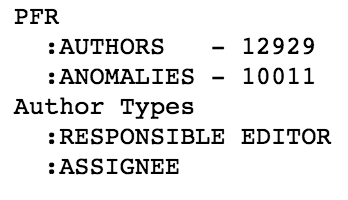
\includegraphics[width=.27\columnwidth]{../images/PFR_count.png}
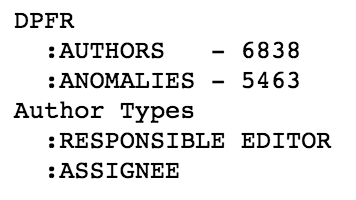
\includegraphics[width=.27\columnwidth]{../images/DPFR_count.png}
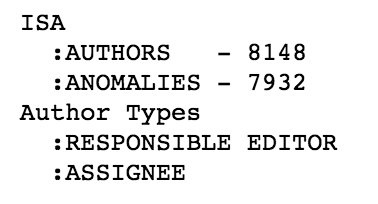
\includegraphics[width=.27\columnwidth]{../images/ISA_count.png}

They\cite{RosenZvi2004}
also state and describe the process for using these single author papers for perplexity.
\begin{quote}
  Perplexity is the standard measure for estimating the performance of a probabilistic model.
\end{quote}
Alternatively, we explore using coherence metrics\cite{Roder2015}, as this has been shown to
provide more understandable topics when applied to bag-of-words topic models. We hope to include
holdout perplexity as a secondary measure, but this is not yet implemented for the model.

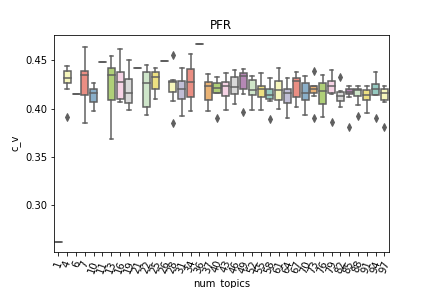
\includegraphics[width=\columnwidth]{../images/PFR_c_v.png}
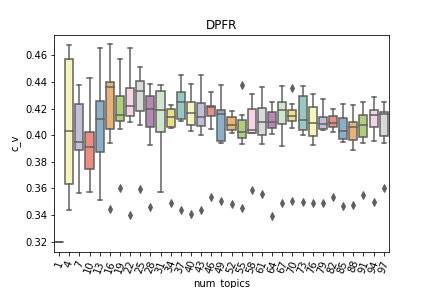
\includegraphics[width=\columnwidth]{../images/DPFR_c_v.png}
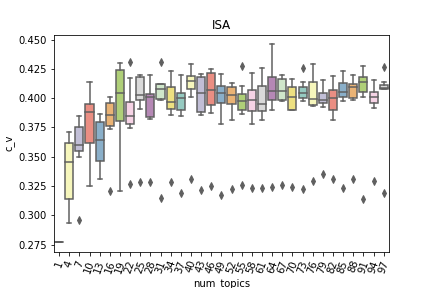
\includegraphics[width=\columnwidth]{../images/ISA_c_v.png}


We also show that the number of publications does not impact model performance, in unexpected ways.

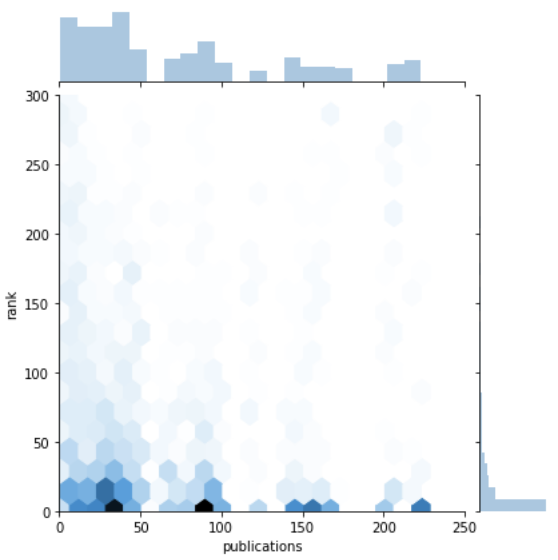
\includegraphics[width=\columnwidth]{../images/Test_pubs.png}
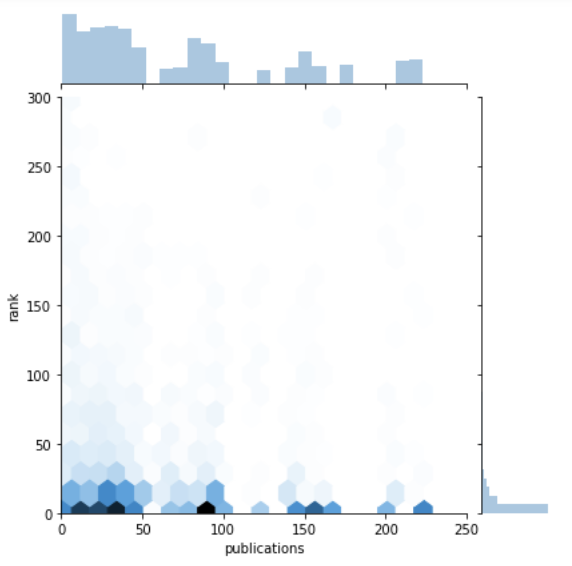
\includegraphics[width=\columnwidth]{../images/Train_pubs.png}

%In my original proposal I suggested an informed train test split by bisecting with
%min-cut\cite{Feige2002} a graph where authors are vertices, and edges exist for each
%co-authors relationship, and is labeled by document name. Unfortunaely our dataset was
%had to few co-attributions to support this.

%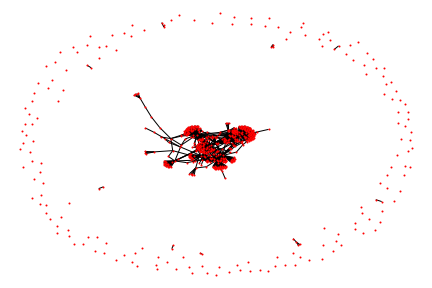
\includegraphics[width=\columnwidth]{../images/PFR_authorship_graph.png}
%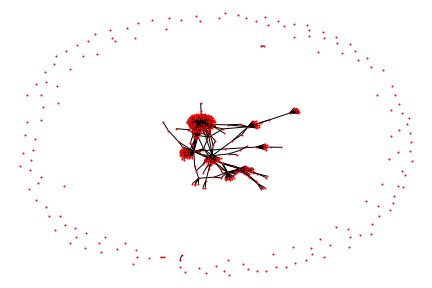
\includegraphics[width=\columnwidth]{../images/DPFR_authorship_graph.png}
%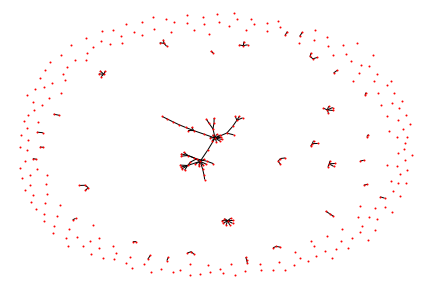
\includegraphics[width=\columnwidth]{../images/ISA_authorship_graph.png}

Later will be important that we investigate the stability of the models\cite{Yang2016}, in order
to incorporate later documents, while minimizing effect to the user experience.


\bibliography{references.bib}{}
\bibliographystyle{plain}
\end{multicols}

\end{document}
